%%%%%%%%%%%%%%%%%%%%%%%%%%%%% Define Article %%%%%%%%%%%%%%%%%%%%%%%%%%%%%%%%%%
\documentclass{article}
%%%%%%%%%%%%%%%%%%%%%%%%%%%%%%%%%%%%%%%%%%%%%%%%%%%%%%%%%%%%%%%%%%%%%%%%%%%%%%%

%%%%%%%%%%%%%%%%%%%%%%%%%%%%% Using Packages %%%%%%%%%%%%%%%%%%%%%%%%%%%%%%%%%%
\usepackage{geometry}
\usepackage{graphicx}
\usepackage{amssymb}
\usepackage{amsmath}
\usepackage{amsthm}
\usepackage{empheq}
\usepackage{mdframed}
\usepackage{booktabs}
\usepackage{lipsum}
\usepackage{listings}
\usepackage{graphicx}
\usepackage{color}
\usepackage{float}
\usepackage{psfrag}
\usepackage{pgfplots}
\usepackage{bm}
%%%%%%%%%%%%%%%%%%%%%%%%%%%%%%%%%%%%%%%%%%%%%%%%%%%%%%%%%%%%%%%%%%%%%%%%%%%%%%%

% Other Settings

\lstset{
  language=R,
  basicstyle=\ttfamily\small,
  keywordstyle=\color{blue}\bfseries,
  commentstyle=\color{green!50!black},
  stringstyle=\color{orange},
  numbers=left,
  numberstyle=\tiny,
  stepnumber=1,
  numbersep=5pt,
  backgroundcolor=\color{gray!10},
  frame=single,
  breaklines=true,
  captionpos=b,
  tabsize=2
}

%%%%%%%%%%%%%%%%%%%%%%%%%% Page Setting %%%%%%%%%%%%%%%%%%%%%%%%%%%%%%%%%%%%%%%
\geometry{a4paper}

%%%%%%%%%%%%%%%%%%%%%%%%%% Define some useful colors %%%%%%%%%%%%%%%%%%%%%%%%%%
\definecolor{ocre}{RGB}{243,102,25}
\definecolor{mygray}{RGB}{243,243,244}
\definecolor{deepGreen}{RGB}{26,111,0}
\definecolor{shallowGreen}{RGB}{235,255,255}
\definecolor{deepBlue}{RGB}{61,124,222}
\definecolor{shallowBlue}{RGB}{235,249,255}
%%%%%%%%%%%%%%%%%%%%%%%%%%%%%%%%%%%%%%%%%%%%%%%%%%%%%%%%%%%%%%%%%%%%%%%%%%%%%%%

%%%%%%%%%%%%%%%%%%%%%%%%%% Define an orangebox command %%%%%%%%%%%%%%%%%%%%%%%%
\newcommand\orangebox[1]{\fcolorbox{ocre}{mygray}{\hspace{1em}#1\hspace{1em}}}
%%%%%%%%%%%%%%%%%%%%%%%%%%%%%%%%%%%%%%%%%%%%%%%%%%%%%%%%%%%%%%%%%%%%%%%%%%%%%%%

%%%%%%%%%%%%%%%%%%%%%%%%%%%% English Environments %%%%%%%%%%%%%%%%%%%%%%%%%%%%%
\newtheoremstyle{mytheoremstyle}{3pt}{3pt}{\normalfont}{0cm}{\rmfamily\bfseries}{}{1em}{{\color{black}\thmname{#1}~\thmnumber{#2}}\thmnote{\,--\,#3}}
\newtheoremstyle{myproblemstyle}{3pt}{3pt}{\normalfont}{0cm}{\rmfamily\bfseries}{}{1em}{{\color{black}\thmname{#1}~\thmnumber{#2}}\thmnote{\,--\,#3}}
\theoremstyle{mytheoremstyle}
\newmdtheoremenv[linewidth=1pt,backgroundcolor=shallowGreen,linecolor=deepGreen,leftmargin=0pt,innerleftmargin=20pt,innerrightmargin=20pt,]{theorem}{Theorem}[section]
\theoremstyle{mytheoremstyle}
\newmdtheoremenv[linewidth=1pt,backgroundcolor=shallowBlue,linecolor=deepBlue,leftmargin=0pt,innerleftmargin=20pt,innerrightmargin=20pt,]{definition}{Definition}[section]
\theoremstyle{myproblemstyle}
\newmdtheoremenv[linecolor=black,leftmargin=0pt,innerleftmargin=10pt,innerrightmargin=10pt,]{problem}{Problem}[section]
%%%%%%%%%%%%%%%%%%%%%%%%%%%%%%%%%%%%%%%%%%%%%%%%%%%%%%%%%%%%%%%%%%%%%%%%%%%%%%%

%%%%%%%%%%%%%%%%%%%%%%%%%%%%%%% Plotting Settings %%%%%%%%%%%%%%%%%%%%%%%%%%%%%
\usepgfplotslibrary{colorbrewer}
\pgfplotsset{width=8cm,compat=1.9}
%%%%%%%%%%%%%%%%%%%%%%%%%%%%%%%%%%%%%%%%%%%%%%%%%%%%%%%%%%%%%%%%%%%%%%%%%%%%%%%

%%%%%%%%%%%%%%%%%%%%%%%%%%%%%%% Title & Author %%%%%%%%%%%%%%%%%%%%%%%%%%%%%%%%
\title{Math 133: Statistical Learning Methods - Module 1 Assessment}
\author{Pranav Jayakumar}
%%%%%%%%%%%%%%%%%%%%%%%%%%%%%%%%%%%%%%%%%%%%%%%%%%%%%%%%%%%%%%%%%%%%%%%%%%%%%%%

\begin{document}
    \maketitle
    \begin{abstract}
      In this module assessment, we will draw from survey data and fit simple linear models to understand the effects of various
      predictors on students' stress. 
    \end{abstract}
    \vspace{0.25in}
    \section{Data Analysis}
    For the following analysis, we will fit simple linear models of the form 
    \[
      Y = \beta_0 + \beta_1X
    \]
    where \textit{Y} = \verb|stress_score| and \textit{X} is one of the following numeric features: \verb|maximum_alcohol_consumed|, \verb|gpa|, or \verb|screen_time|. 
    \vspace{0.1in}
    \subsection{Data Visualization}
    We will begin by creating scatterplots of students' stress scores vs. each of the three aforementioned predictors.
    We will use a 70-30 training-testing split for our models.
    \vspace{0.1in}
    \begin{figure}[H]
      \begin{center}
        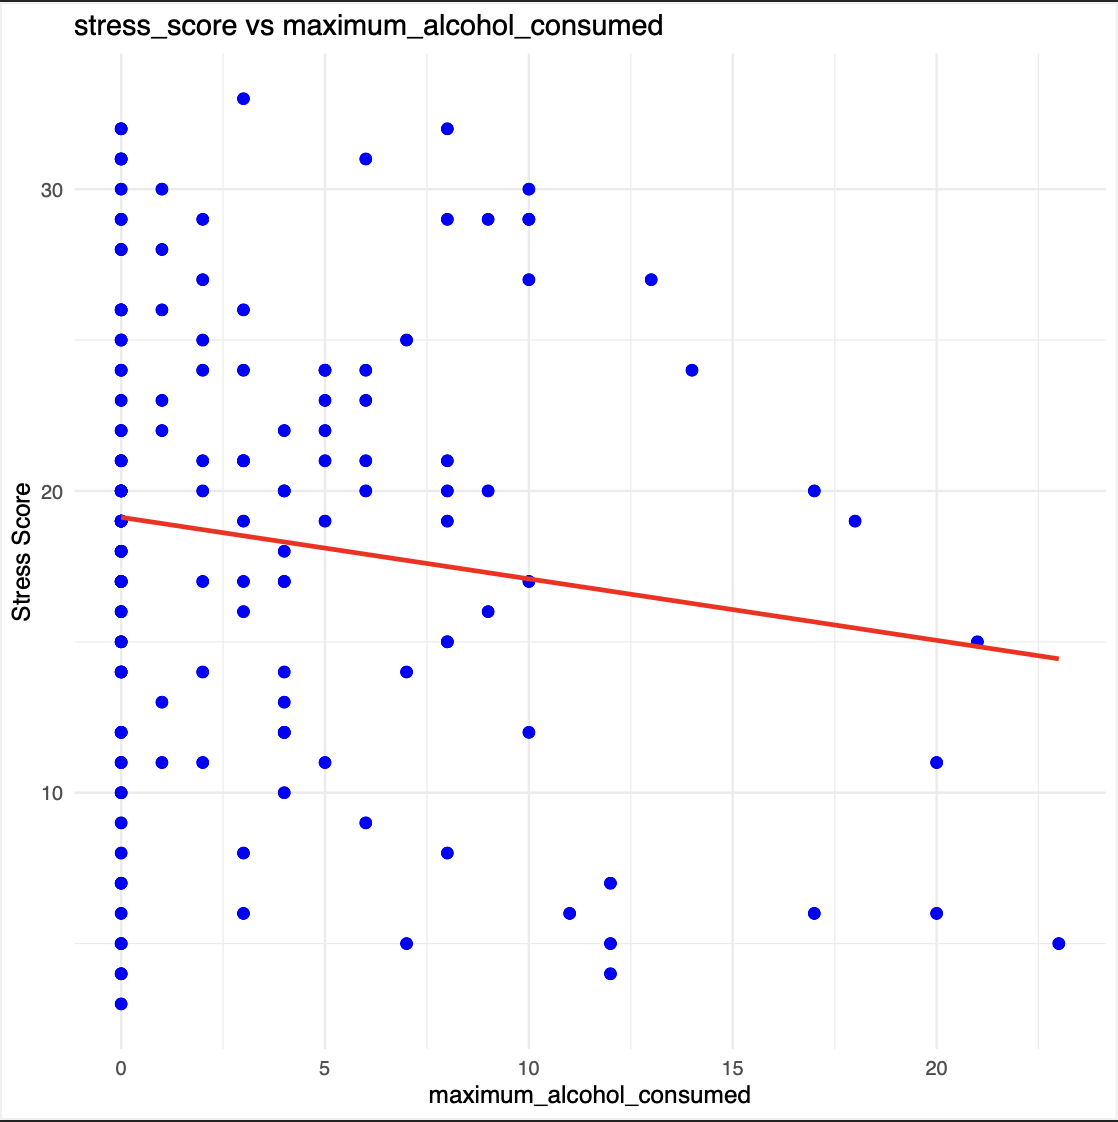
\includegraphics[width=0.45\textwidth]{figures/stress_vs_alcohol.png}
      \end{center}
      \caption{Scatterplot of Stress Score vs. Maximum Alcohol Consumed}\label{fig:}
    \end{figure}
    
    The linear model for stress score vs. maximum alcohol consumed is represented by:
    \[\hat{y} = 18.8543 -0.2999x\]
    We observe an \(R^2\) score of 0.0417.  
    \vspace{0.1in}
    \begin{figure}[H]
    \begin{center}
      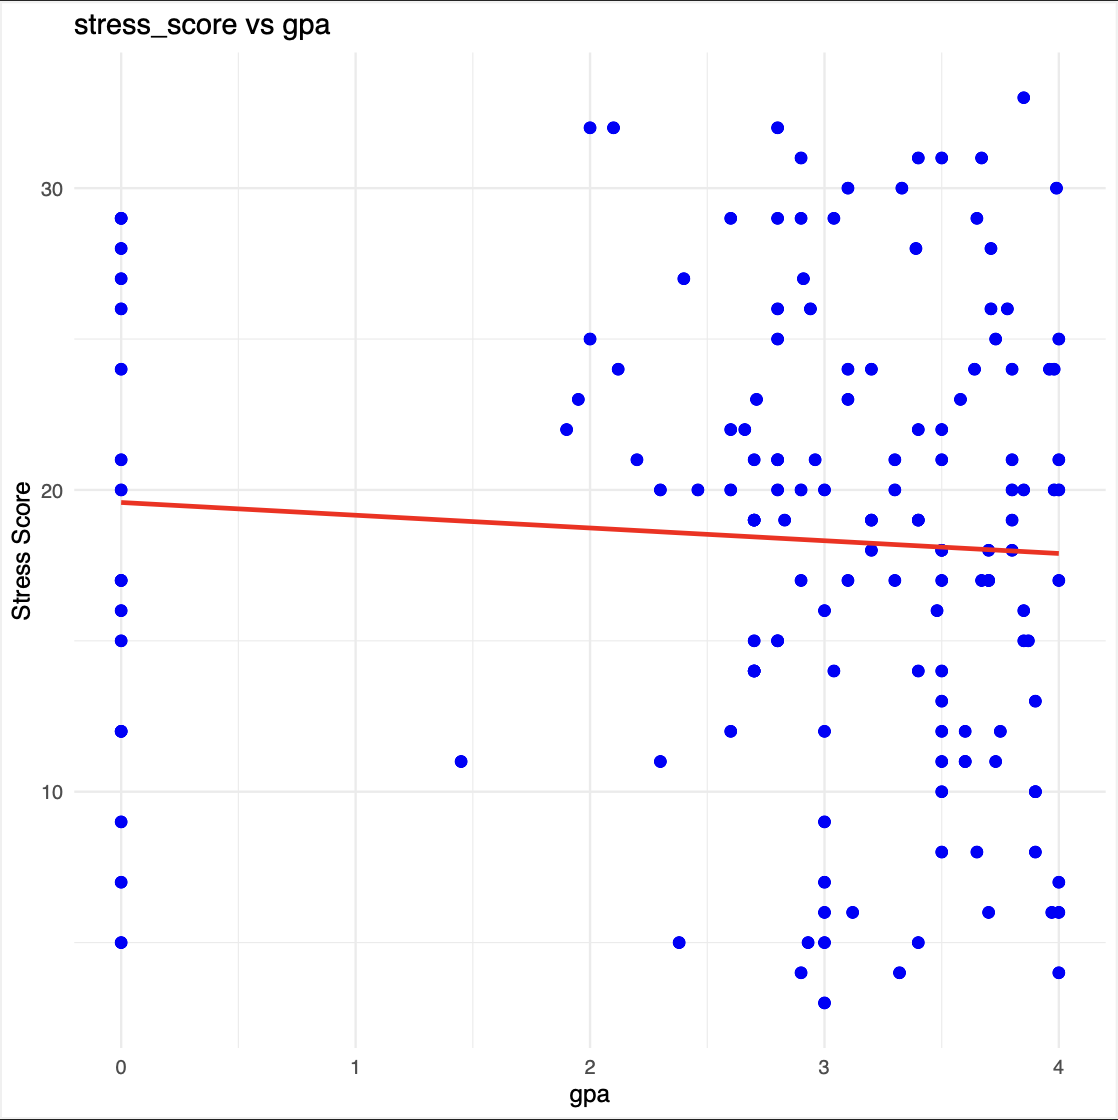
\includegraphics[width=0.45\textwidth]{figures/stress_vs_gpa.png}
    \end{center}
    \caption{Scatterplot of Stress Score vs. GPA}\label{fig:}
  \end{figure}
  
  The linear model for stress score vs. GPA is represented by:
  \[\hat{y} = 19.8029 -0.3343x\]
  We observe an \(R^2\) score of 0.0027. 
  \vspace{0.1in}
  \begin{figure}[H]
    \begin{center}
      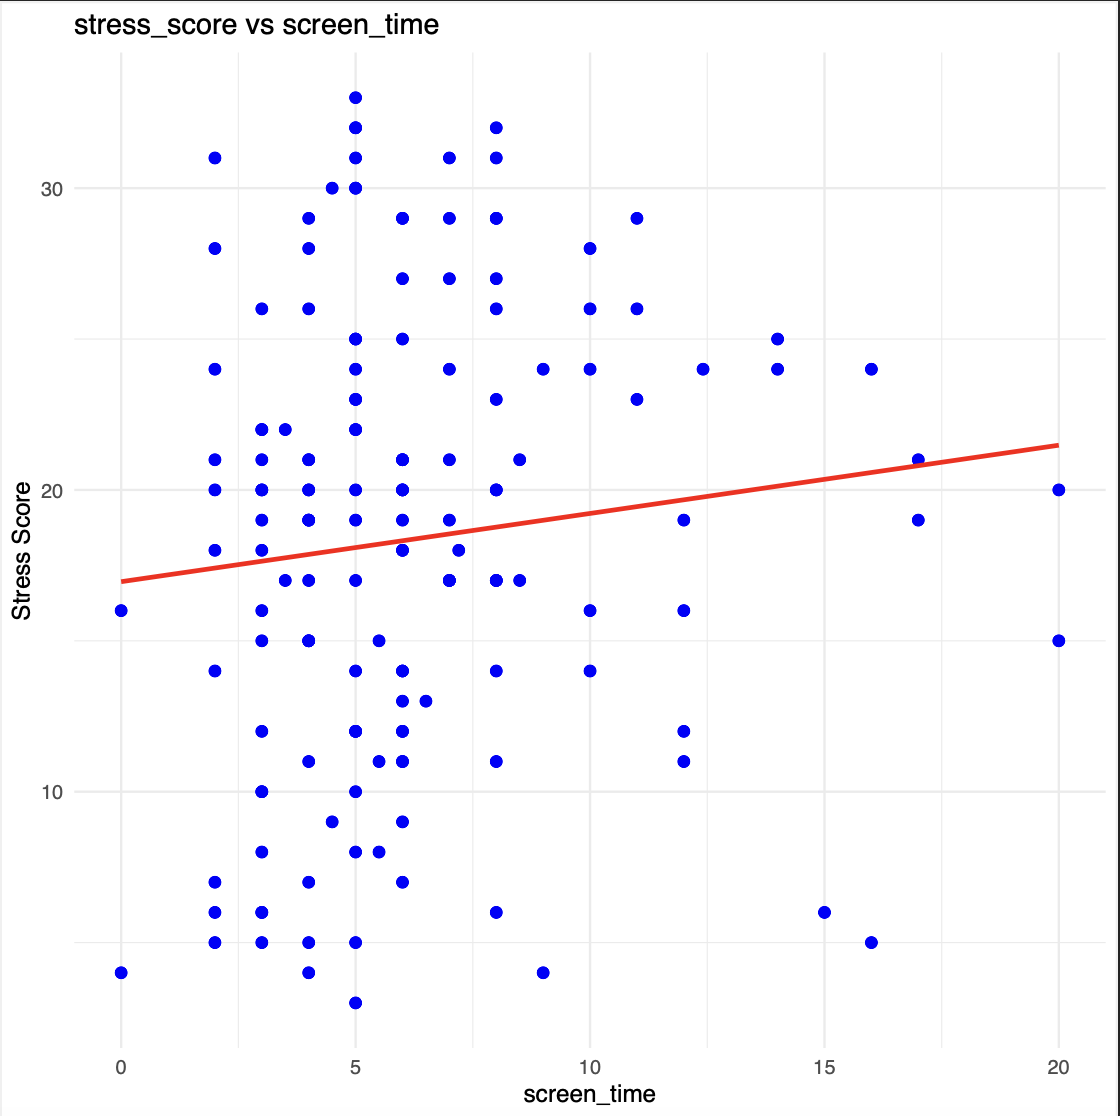
\includegraphics[width=0.45\textwidth]{figures/stress_vs_screentime.png}
    \end{center}
    \caption{Scatterplot of Stress Score vs. Screen Time}\label{fig:}
  \end{figure}

  The linear model for stress score vs. screen time is represented by:
  \[\hat{y} = 16.7664 + 0.3193x\]
  We observe an \(R^2\) score of 0.0222. 
  \vspace{0.25in}
  \subsection{Insights}

  We observe that the linear model \verb|stress_score~screen_time| has the highest \(R^2\) score. 
  Therefore, there is evidence to suggest that screen time is the best out of the three predictors of stress.\\ 
  \\ 
  Plotting screen time data in a histogram shows that the data is approximately normally distributed.
  \vspace{0.1in}
  \begin{figure}[H]
    \begin{center}
      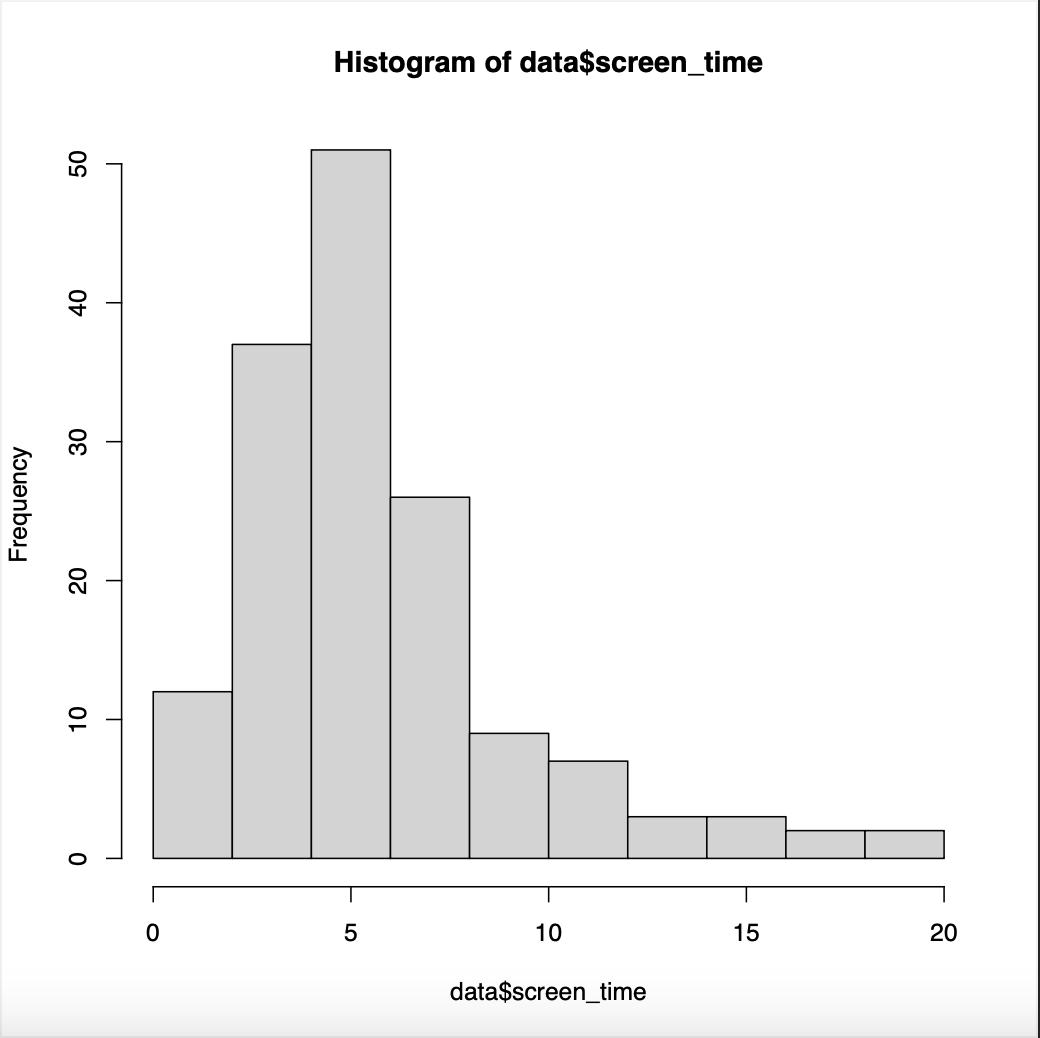
\includegraphics[width=0.45\textwidth]{figures/screentime_histogram.png}
    \end{center}
    \caption{Histogram of Screen Time}\label{fig:}
  \end{figure}

  \section{R Coding}
  \begin{lstlisting}
    #!/usr/bin/env Rscript
library(ggplot2)

set.seed(123)

fit_linear_model <- function(y, x, raw_data) {
  # Train-test split
  n <- nrow(raw_data)
  trainIndex <- sample(n, round(0.7 * n, 0))
  train <- raw_data[trainIndex, ]
  test <- raw_data[-trainIndex, ]
  
  # Construct formula
  formula <- as.formula(paste(y, "~", x))
  
  # Fit model
  model <- lm(formula, data = train)

  overview = summary(model)
  print(overview)
  
  # Predict on testing data
  y_test <- test[[y]]
  y_hat <- predict(model, newdata = test)
  
  # Analyze accuracy
  SSE <- sum((y_test - y_hat)^2)
  MSE <- SSE / nrow(test)  
  RMSE <- sqrt(MSE)
  SST <- sum((y_test - mean(y_test))^2)
  R2 <- 1 - SSE / SST
  
  return(list(SSE = SSE, MSE = MSE, RMSE = RMSE, SST = SST, R2 = R2))
}

main <- function() {
  # Load data
  data <- read.csv("../../data/survey_fall2023.csv")
  
  # Define predictors
  predictors <- c("maximum_alcohol_consumed", "gpa", "screen_time")
  results <- list()
  
  # Open PDF device for saving all plots
  pdf("Rplots.pdf")  # This will save all plots sequentially to Rplots.pdf
  
  # Iterate over predictors
  for (predictor in predictors) {
    if (!predictor %in% colnames(data)) {
      cat("\nWarning: Predictor", predictor, "not found in dataset. Skipping...\n")
      next
    }
    
    cat("\nLinear model for stress score ~", predictor, "\n")
    result <- fit_linear_model("stress_score", predictor, data)
    
    # Store results for later comparison
    results[[predictor]] <- result
    
    # Format and print results
    formatted_results <- lapply(result[1:5], function(x) format(round(x, 4), nsmall = 4))
    print(formatted_results)
    
    # Create scatterplot for the predictor
    ggplot(data, aes_string(x = predictor, y = "stress_score")) +
      geom_point(color = "blue", size = 2) +
      geom_smooth(method = "lm", color = "red", se = FALSE) +
      ggtitle(paste("stress_score vs", predictor)) +
      xlab(predictor) +
      ylab("Stress Score") +
      theme_minimal() -> plot  # Assign ggplot to a variable

    print(plot)  # Ensure the plot is sent to the PDF file
  }

  hist(data$screen_time, breaks = "Freedman-Diaconis") -> plot1
  print(plot1)
  
  # Close PDF device
  dev.off()
  
  cat("\nAll plots saved to Rplots.pdf.\n")
}

# Run the script if executed directly
if (interactive() || identical(Sys.getenv("R_SCRIPT"), "")) {
  main()
}
\end{lstlisting}


  
\end{document}
